% -*- latex -*-
%%%%%%%%%%%%%%%%%%%%%%%%%%%%%%%%%%%%%%%%%%%%%%%%%%%%%%%%%%%%%%%%
%%%%%%%%%%%%%%%%%%%%%%%%%%%%%%%%%%%%%%%%%%%%%%%%%%%%%%%%%%%%%%%%
%%%%
%%%% This text file is part of the source of slides for
%%%% `Introduction to High-Performance Scientific Computing'
%%%% by Victor Eijkhout, copyright 2012
%%%%
%%%%%%%%%%%%%%%%%%%%%%%%%%%%%%%%%%%%%%%%%%%%%%%%%%%%%%%%%%%%%%%%
%%%%%%%%%%%%%%%%%%%%%%%%%%%%%%%%%%%%%%%%%%%%%%%%%%%%%%%%%%%%%%%%


%\usepackage{graphicx,comment,multicol,undertilde}
%\usepackage{amsmath,arydshln}


\frame{\frametitle{Boundary value problems}
  Consider in 1D
\[ 
\begin{cases}
  -u''(x)=f(x,u,u')&x\in[a,b]\\
  u(a)=u_a,\,u(b)=u_b
\end{cases}
\]
in 2D:
\[
\begin{cases}
  -u_{xx}(\bar x)-u_{yy}(\bar x)=f(\bar x)&x\in\Omega=[0,1]^2\\
  u(\bar x)=u_0&\bar x\in\delta\Omega
\end{cases}
\]
}

\frame{\frametitle{Approximation of 2nd order derivatives}
\footnotesize
  Taylor series (write $h$ for $\delta x$):
  \[ u(x+h)=u(x)+u'(x)h+u''(x)\frac{h^2}{2!}+u'''(x)\frac{h^3}{3!}
  +u^{(4)}(x)\frac{h^4}{4!}+u^{(5)}(x)\frac{h^5}{5!}+\cdots \]
  and
  \[ u(x-h)=u(x)-u'(x)h+u''(x)\frac{h^2}{2!}-u'''(x)\frac{h^3}{3!}
  +u^{(4)}(x)\frac{h^4}{4!}-u^{(5)}(x)\frac{h^5}{5!}+\cdots \]
  Subtract:
  \[ u(x+h)+u(x-h)=2u(x)+u''(x)h^2+u^{(4)}(x)\frac{h^4}{12}+\cdots \]
  so
  \[ u''(x)=\frac{u(x+h)-2u(x)+u(x-h)}{h^2}-u^{(4)}(x)\frac{h^4}{12}+\cdots \]


  Numerical scheme:
  \[ -\frac{u(x+h)-2u(x)+u(x-h)}{h^2}=f(x,u(x),u'(x)) \]
  (2nd order PDEs are very common!)
}

\frame{\frametitle{This leads to linear algebra}
  \[ -u_{xx}=f\rightarrow
  \frac{2u(x)-u(x+h)-u(x-h)}{h^2}=f(x,u(x),u'(x)) 
  \]
  Equally spaced points on $[0,1]$: $x_k=kh$ where $h=1/(n+1)$, then
  \[ -u_{k+1}+2u_k-u_{k-1} = -1/h^2\,f(x_k,u_k,u'_k)
  \quad\hbox{for $k=1,\ldots,n$} \]
  Written as matrix equation:
  \[
  \left(
    \begin{matrix}
      2&-1\\ -1&2&-1\\ &\ddots&\ddots&\ddots
    \end{matrix}\right)
  \left(
    \begin{matrix}
      u_1\\ u_2\\ \vdots
    \end{matrix}\right)
  =
  \left(
    \begin{matrix}
      f_1+u_0\\ f_2\\ \vdots
    \end{matrix}\right)
  \]
}

\frame{\frametitle{Matrix properties}

  \begin{itemize}
  \item Very sparse, banded
  \item Symmetric (only because 2nd order problem)
  \item Sign pattern: positive diagonal, nonpositive off-diagonal\\
    (true for many second order methods)
  \item Positive definite (just like the continuous problem)
  \item Constant diagonals (from constant coefficients in the DE)
  \end{itemize}
}

\frame{\frametitle{Sparse matrix in 2D case}
\small
Sparse matrices so far were tridiagonal: only in 1D case.

Two-dimensional: $-u_{xx}-u_{yy}=f$ on unit square $[0,1]^2$

Difference equation: 
 \[ 4u(x,y)-u(x+h,y)-u(x-h,y)-u(x,y+h)-u(x,y-h)=h^2f(x,y) \]

\[ 4u_k-u_{k-1}-u_{k+1}-u_{k-n}-u_{k+n}=f_k \]
Consider a graph where $\{u_k\}_k$ are the edges\\
and $(u_i,u_j)$ is an edge iff $a_{ij}\not=0$.
}

\frame{\frametitle{The graph view of things}
Poisson eq:
\centerline{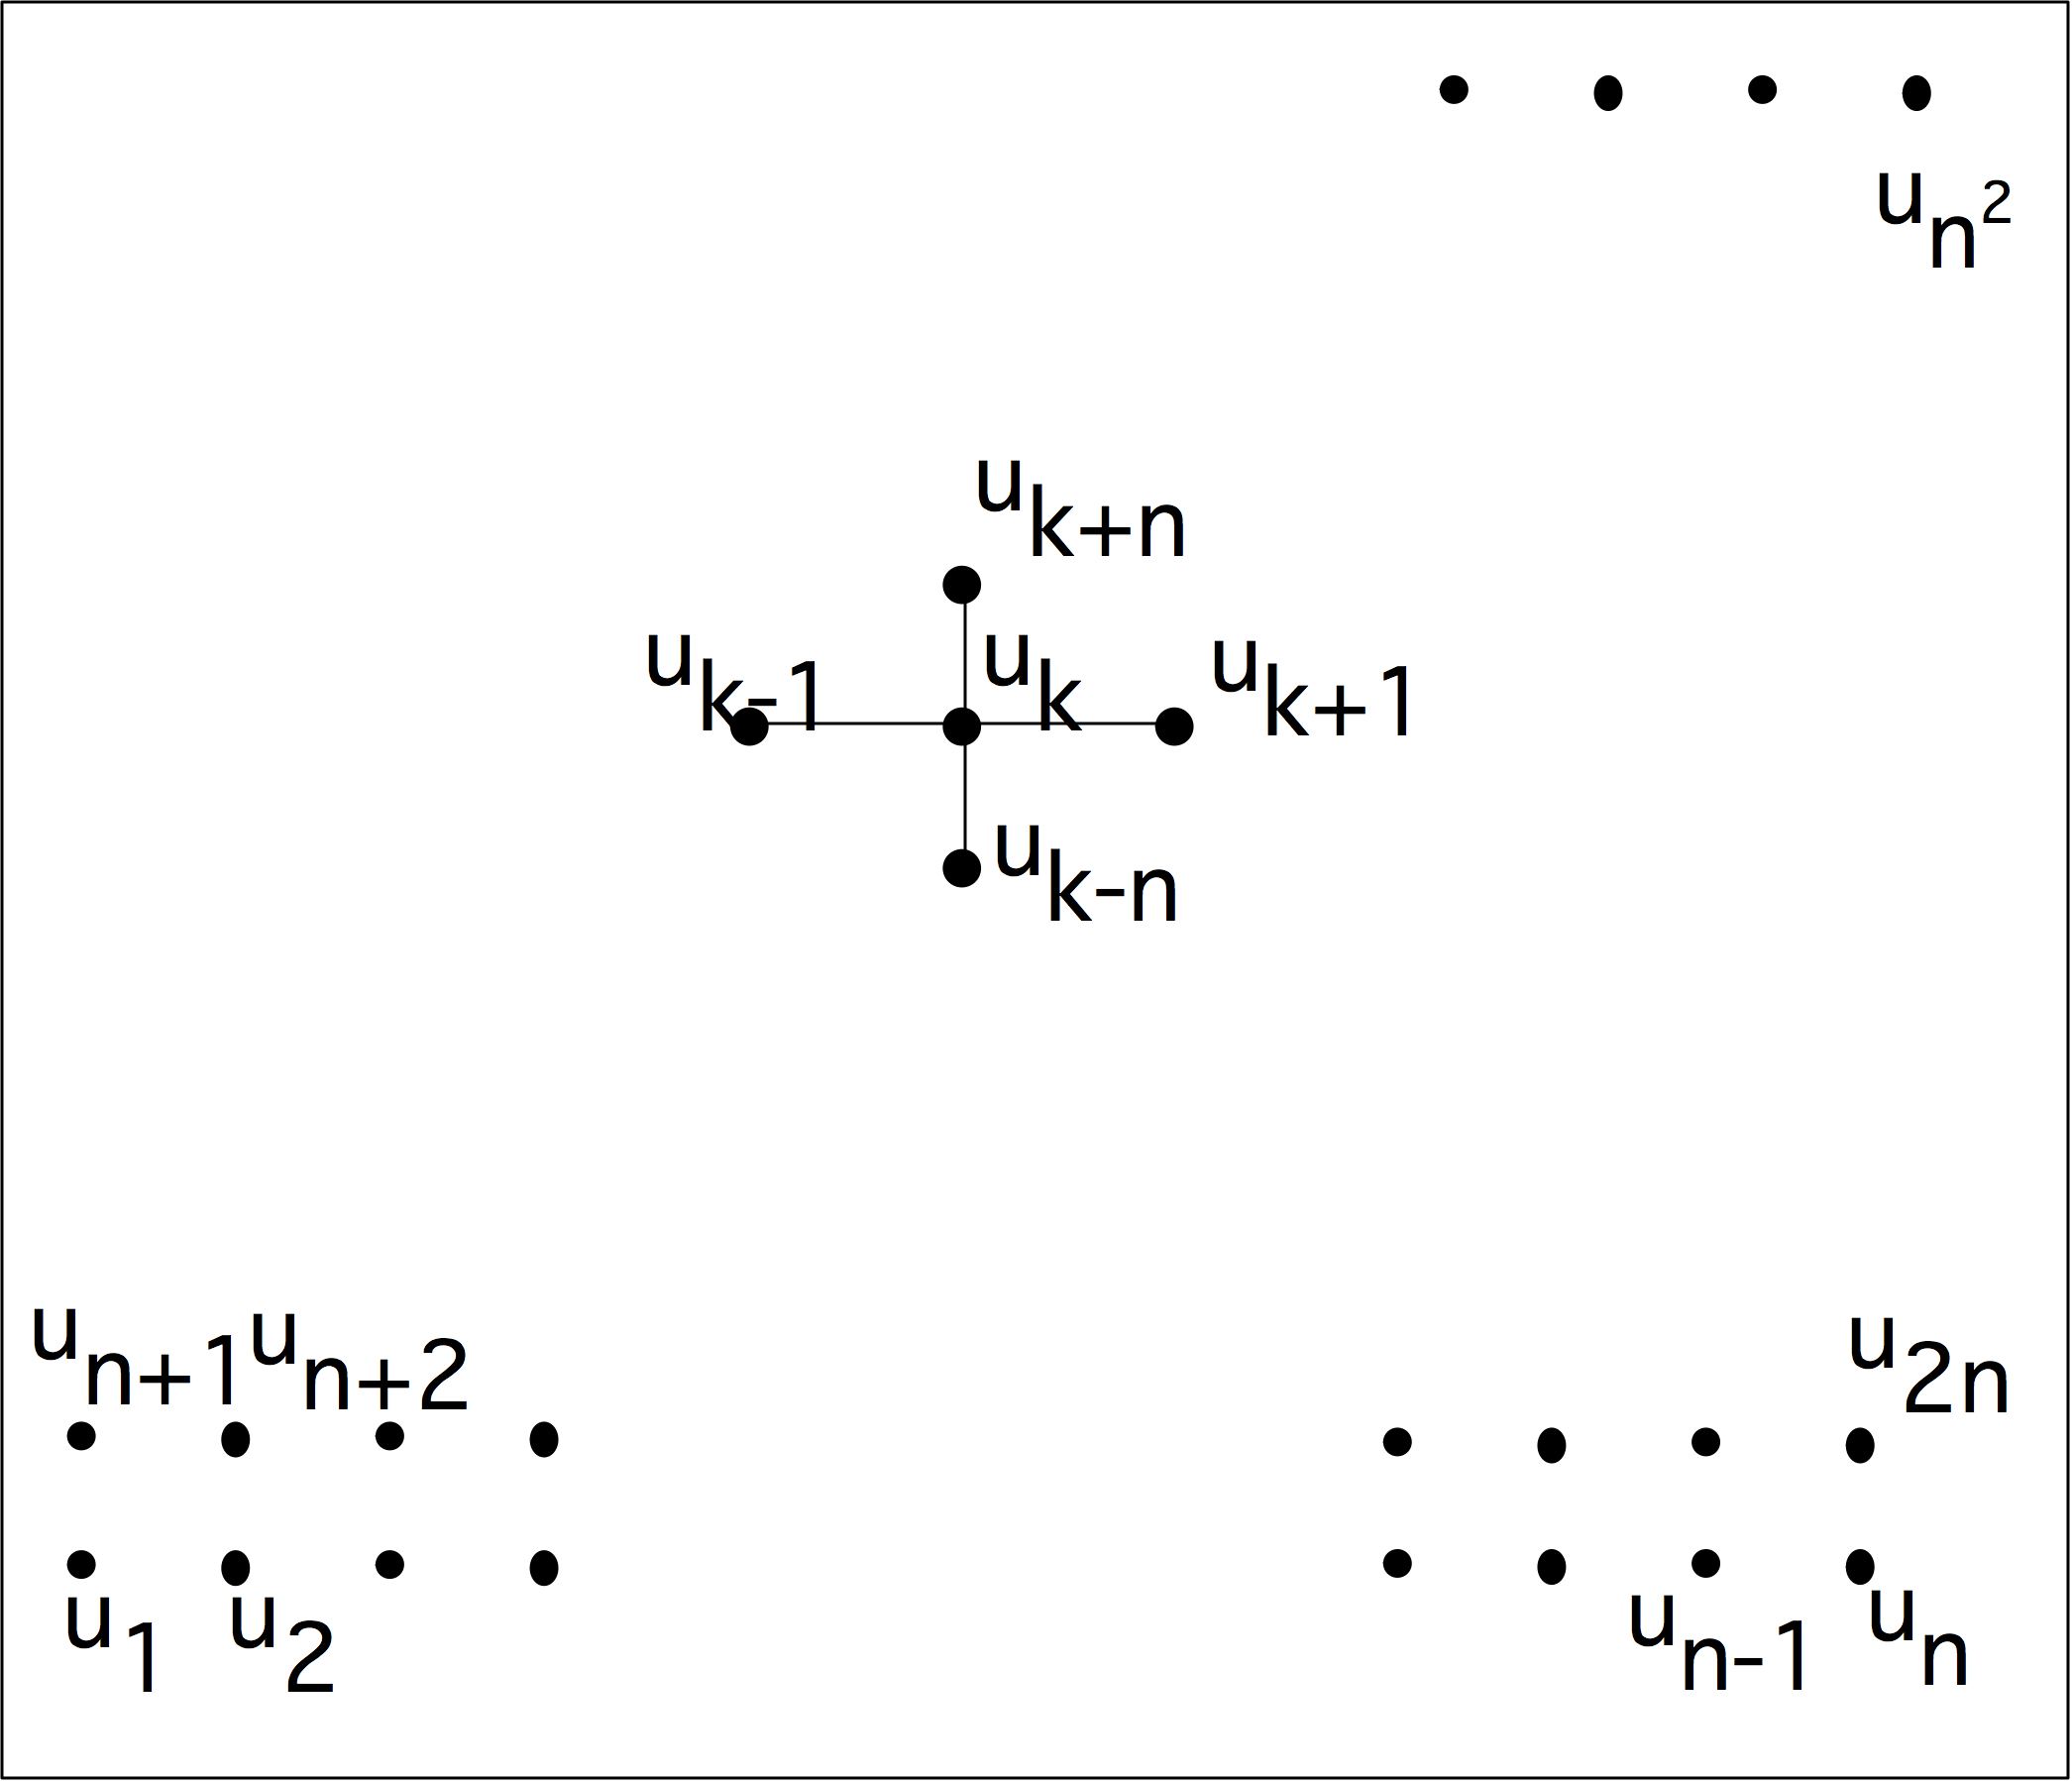
\includegraphics[scale=.07]{laplacedomain}
\hskip10pt\parbox{2in}{This is a graph!}}
This is the (adjacency) graph of a sparse matrix.
}

\frame{\frametitle{Sparse matrix from 2D equation}
\small
\[
  \left(\begin{array}{ccccc|ccccc|cc}
    4&-1&&&\emptyset&-1&&&&\emptyset&\\ 
    -1&4&1&&&&-1&&&&\\ 
    &\ddots&\ddots&\ddots&&&&\ddots&&\\ 
    &&\ddots&\ddots&-1&&&&\ddots&\\ 
    \emptyset&&&-1&4&\emptyset&&&&-1&\\ \hline
    -1&&&&\emptyset&4&-1&&&&-1\\
    &-1      &      &&&-1      &4       &-1      &&&&-1\\
    &\uparrow&\ddots&&&\uparrow&\uparrow&\uparrow&&  &&\uparrow\\
    &k-n     &      &&&k-1     &k       &k+1     &&-1&&k+n\\
    &&&&-1&&&&-1&4&&\\ \hline
    &        &      &&&\ddots  &        &        &&  &\ddots\\
  \end{array}\right)
\]
}


\frame{\frametitle{Matrix properties}

  \begin{itemize}
  \item Very sparse, banded
  \item Factorization takes less than $n^2$ space, $n^3$~work
  \item Symmetric (only because 2nd order problem)
  \item Sign pattern: positive diagonal, nonpositive off-diagonal\\
    (true for many second order methods)
  \item Positive definite (just like the continuous problem)
  \item Constant diagonals: only because of the constant coefficient
    differential equation
  \item Factorization: lower complexity than dense, recursion length less than~$N$.
  \end{itemize}
}

\frame{\frametitle{Realistic meshes}
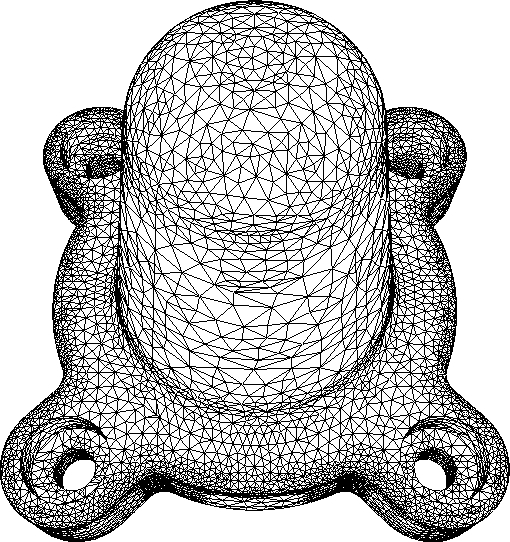
\includegraphics[scale=.3]{img206}
%
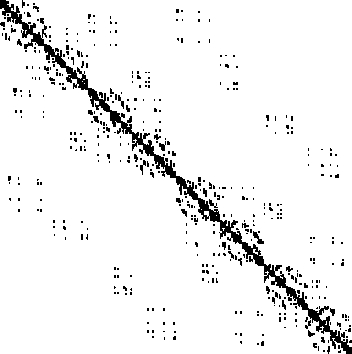
\includegraphics[scale=.3]{sparse-example}
}

